% Chapter Template

\chapter{Ensayos y resultados} % Main chapter title

\label{Chapter4} % Change X to a consecutive number; for referencing this chapter elsewhere, use \ref{ChapterX}

En este capítulo se explica cómo se hicieron los ensayos y qué resultados se obtuvieron.
%----------------------------------------------------------------------------------------
%	SECTION 1
%----------------------------------------------------------------------------------------

\section{Banco de pruebas}
\label{sec:entornos}

Se utilizaron 3 entornos para llevar a cabo el desarrollo y las consecuentes pruebas del sistema. A nivel de \textit{software} se administraron utilizando un repositorio en la nube y manteniendo 3 ramas individuales de código, una para cada entorno. A nivel de \textit{hardware} se fue escalando entre entornos a medida que se avanzaba en el desarrollo y las pruebas.

Los entornos se denominaron de la siguiente manera:
\begin{itemize}
\item dev: para referirse a \textit{development} o desarrollo.
\item test: para referirse a \textit{testing} o pruebas.
\item prod: para referirse a \textit{production} o producción.
\end{itemize}

En la figura \ref{fig:entornos} podemos observar cada entorno y las tareas realizadas en cada uno.

\begin{figure}[H]
	\centering
	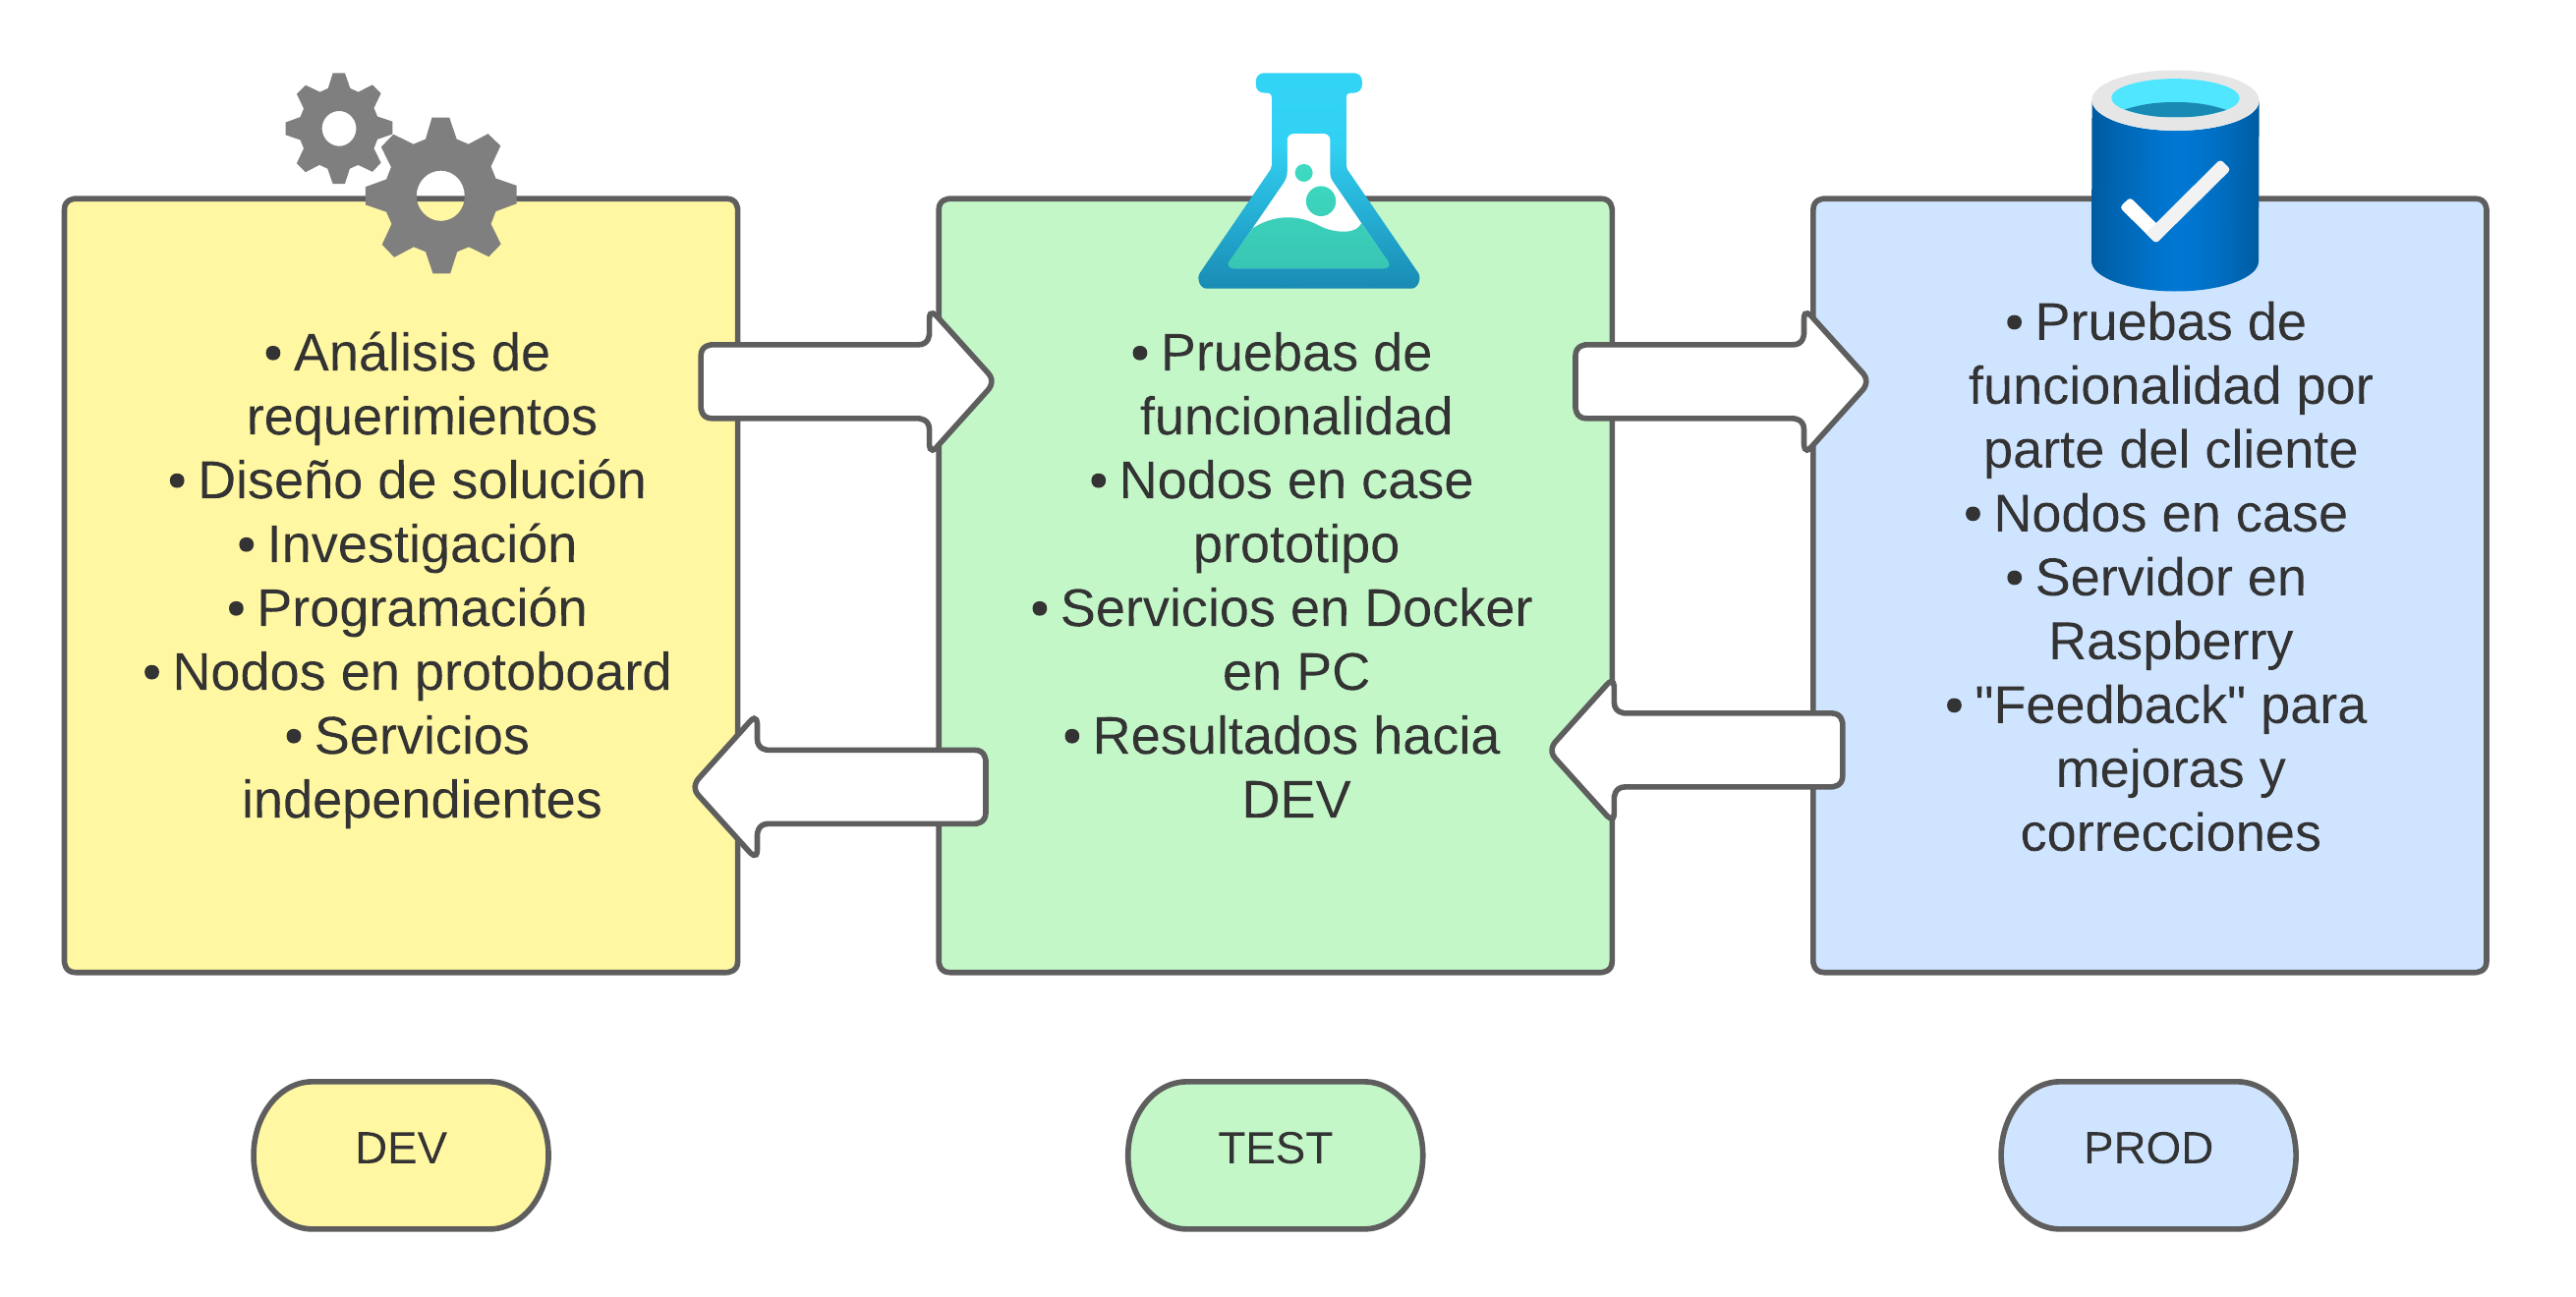
\includegraphics[scale=.15]{./Figures/diagrama-entornos.png}
	\caption{Entornos de desarrollo y pruebas del sistema.}
	\label{fig:entornos}
\end{figure}

\section{Ensayos sobre la API}
\label{sec:ensayos-api}

Para realizar las pruebas en las comunicaciones HTTP y validar la funcionalidad de la API de \textit{backend} y la API \textit{messenger}, se utilizó la herramienta de prueba de API llamada Insomnia, la cual permite hacer solicitudes utilizando los métodos HTTP.

Se creó la estructura de \textit{endpoints} del sistema separadas en carpetas y archivos según módulos o funcionalidad y se declararon los diferentes entornos de prueba (\textit{dev, test y prod}) descritos en la sección anterior. 

Se realizaron diversas pruebas como: la autenticación de usuario, la validación de parámetros de solicitud, el manejo de errores, las respuestas del servidor, la manipulación de datos en la base de datos y la integración de servicios de terceros, entre otras.

En las figuras \ref{fig:insomnia-carpetas} se muestra un ejemplo de la estructura de carpetas utilizadas y sus rutas, se pueden ver los métodos HTTP y el entorno utilizado, en este caso, \textit{dev localhost}.

\begin{figure}[H]
	\centering
	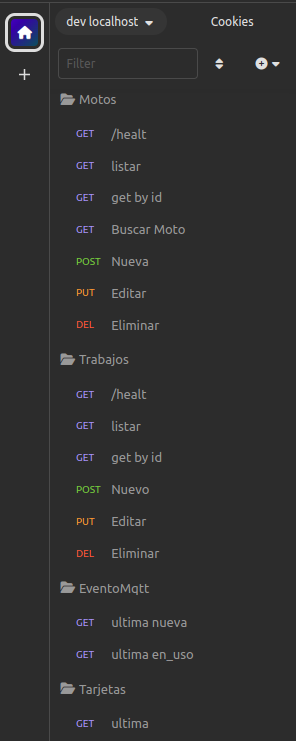
\includegraphics[scale=.50]{./Figures/insomnia-carpetas2.png}
	\caption{Estructura de carpetas y archivos en Insomnia.}
	\label{fig:insomnia-carpetas}
\end{figure}
  
En la figura \ref{fig:insomnia-request-1} podemos observar un ejemplo de una petición HTTP GET a la ruta para filtrar órdenes de trabajo.

\begin{figure}[H]
	\centering
	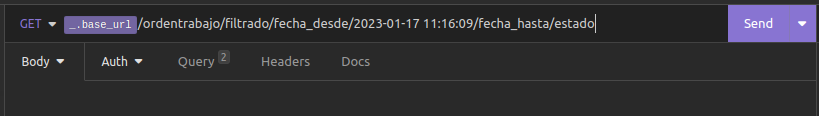
\includegraphics[width=\textwidth]{./Figures/insomnia-request-1.png}
	\caption{Estructura de carpetas y archivos en Insomnia.}
	\label{fig:insomnia-request-1}
\end{figure}

El parámetro \textit{base url} es una variable de entorno que trae la ruta base según el entorno en que estemos trabajando, en este caso el entorno es \textit{dev localhost} y la variable \textit{http://localhost:3001}. Observamos la ruta y los parámetros en la URL. Se pueden añadir el \textit{body} y \textit{header} de la petición así como también el \textit{token} de autenticación.

En la figura \ref{fig:insomnia-request-2} vemos la respuesta a la petición, dónde se indica el código de \textit{status} HTTP, en este caso 200, el tiempo de respuesta en milisegundos y el tamaño de la respuesta en \textit{Kilobytes}. En la pestaña \textit{Preview} muestra el resultado de la petición en formato JSON y se pueden ver en las siguiente pestañas el \textit{header, cookies y timeline} de la respuesta. 

\begin{figure}[H]
	\centering
	\includegraphics[scale=.45]{./Figures/insomnia-request-2.png}
	\caption{Respuesta de una petición en Insomnia.}
	\label{fig:insomnia-request-2}
\end{figure}


\section{Ensayos sobre el sistema}
\label{sec:ensayos-nodos}

Primeramente, durante la etapa de desarrollo \textit{dev} y \textit{test}, se fueron realizando pruebas a medida que se avanzaba en el desarrollo. Para esto se utilizaron placas de prototipo \textit{protoboard} para los nodos y se ejecutaron los sistemas en modo local utilizando Nodemon y posteriormente Docker y Docker Compose, como se describe en la sección \ref{sec:entornos} del presente capítulo.

Luego de superadas las pruebas iniciales se procedió a las pruebas funcionales del sistema. Estas se realizaron sobre el sistema completo en ejecución, ya que todas las partes del sistema interactúan entre sí. 

Una vez que se conectaron todos los nodos y el servidor Raspberry Pi a la corriente eléctrica se realizaron las pruebas en el sistema web. Se realizó el recorrido completo del proceso de una órden de trabajo mientras se analizaba en paralelo las terminales de línea de comandos y la funcionalidad \textit{debug} del navegador.

Para comprobar el estado del servidor y de cada servicio se utilizó el servicio Portainer en donde se accedió a los logs de cada contenedor directamente.

\subsection{Inicio del servidor}
\label{subsec:ensayoservidor}

Como primera medida comprobamos el estado del servidor y sus servicios. En la figura \ref{fig:ensayoportainer3} podemos observar el estado de los contenedores, su nombre, dirección IP, puertos, entre otros datos.

\begin{figure}[H]
	\centering
	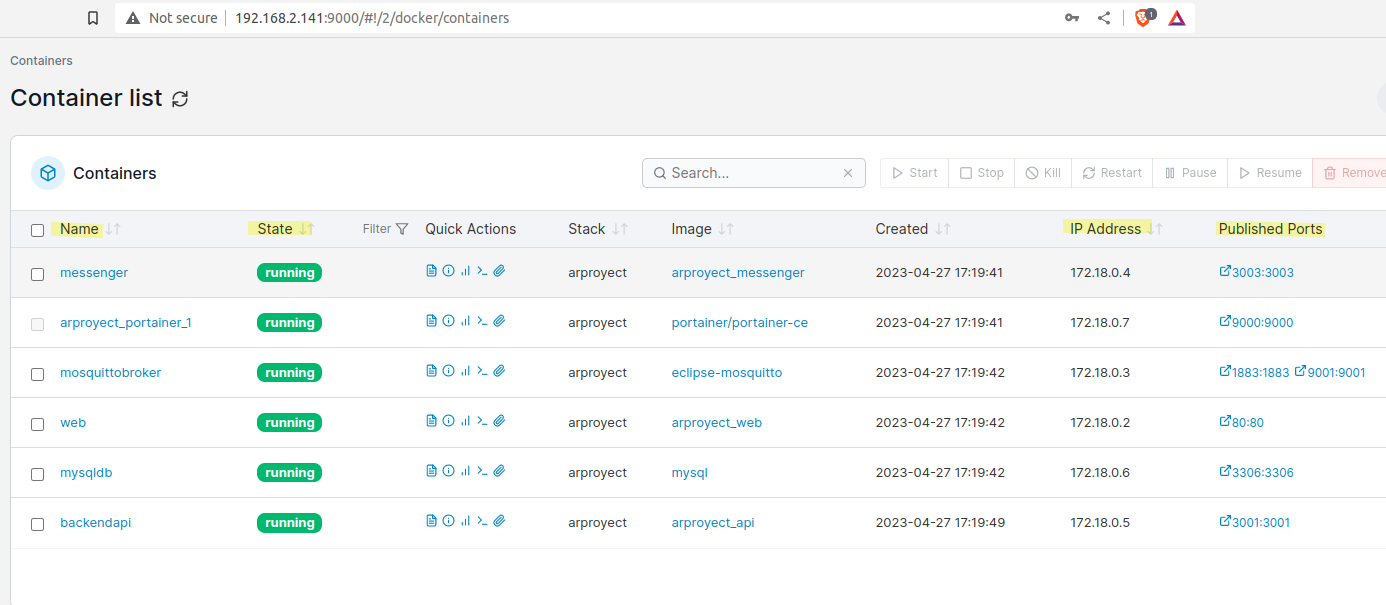
\includegraphics[scale=.35]{./Figures/ensayo-1/3.portainer.png}
	\caption{Estado de contenedores.}
	\label{fig:ensayoportainer3}
\end{figure}

Ingresamos a los \textit{logs} del servicio de la API \textit{backend} para verificar su funcionamiento.  En la figura \ref{fig:ensayoportainerlogapi} podemos observar los registros del \textit{log}.

\begin{figure}[H]
	\centering
	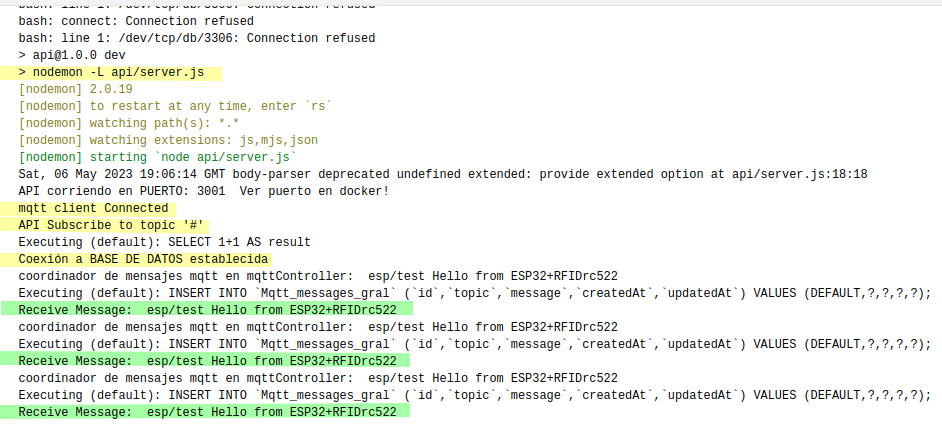
\includegraphics[width=\textwidth]{./Figures/ensayo-1/4.portainer-log-api.png}
	\caption{Estado de contenedores.}
	\label{fig:ensayoportainerlogapi}
\end{figure}

Resaltado con amarillo podemos observar la ejecución del log con Nodemon, el mensaje de conexión correcta al \textit{broker} MQTT, la suscripción a todos los tópicos y la conexión correcta a la base de datos.

Resaltado en color verde podemos observar 3 líneas similares. Cada una de estas líneas corresponde a cada nodo enviando un mensaje de confirmación a la API, de esta manera podemos comprobar que los 3 nodos se conectaron correctamente al \textit{broker} MQTT. 

\subsection{Carga de nueva órden de trabajo}
\label{subsec:ensayonuevaorden}

En la figura \ref{fig:ensayonueva1} podemos ver el inicio del proceso para el ingreso de una nueva órden de trabajo. Observamos una vista general que luego ampliaremos para analizarla mejor.

\begin{figure}[H]
	\centering
	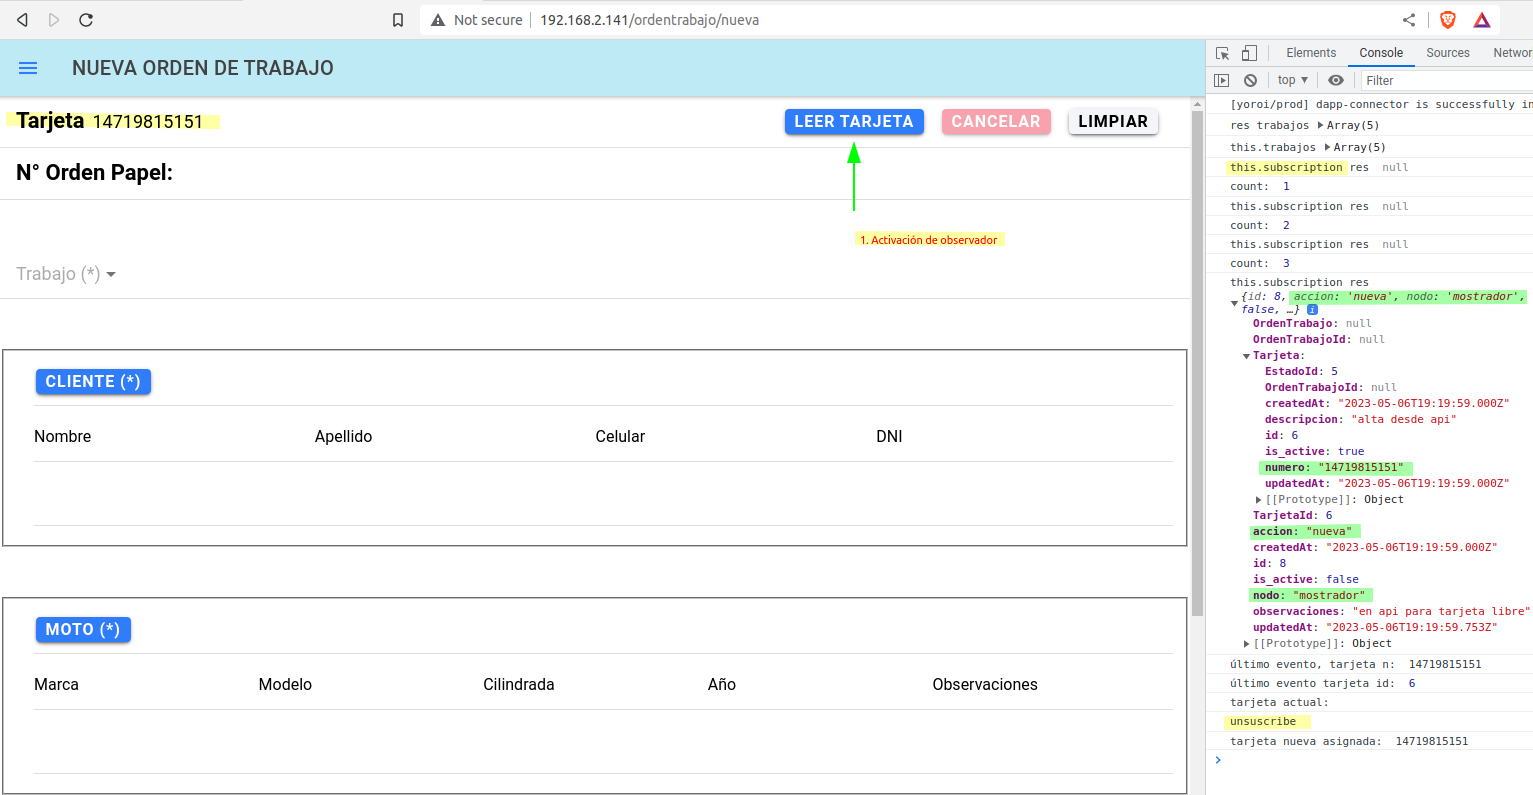
\includegraphics[width=\textwidth]{./Figures/ensayo-1/5.nueva.png}
	\caption{Interfaz para carga de nueva órden de trabajo.}
	\label{fig:ensayonueva1}
\end{figure}

En la figura \ref{fig:ensayonueva1-1} vemos en detalle la sección donde se activa la función observador de Ionic para luego pasar la tarjeta por el nodo \textit{mostrador}. Una vez que pasamos la tarjeta por el lector aparecé el número de tarjeta que, para este ejemplo, está resaltado en color amarillo.

\begin{figure}[H]
	\centering
	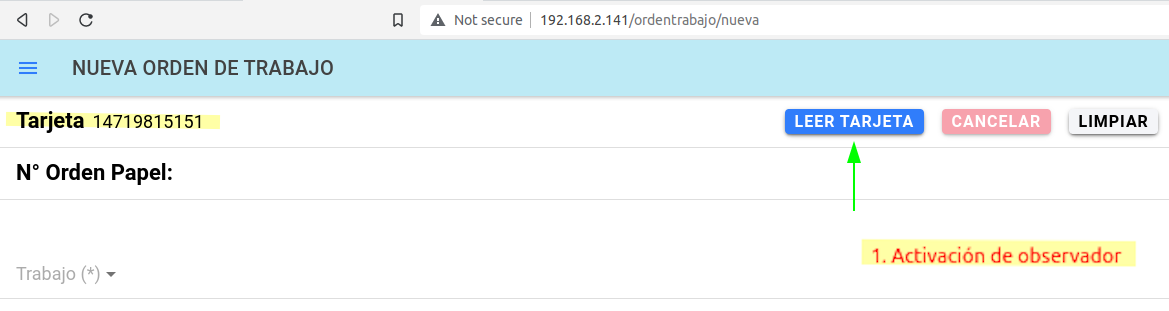
\includegraphics[width=\textwidth]{./Figures/ensayo-1/5.nueva-1.png}
	\caption{Interfaz para carga de nueva órden de trabajo.}
	\label{fig:ensayonueva1-1}
\end{figure}

En la figura \ref{fig:ensayonueva1-2} podemos observar la sección \textit{debug} del navegador donde podemos ver los mensajes que dejamos en el código fuente para hacer análisis del sistema.

\begin{figure}[H]
	\centering
	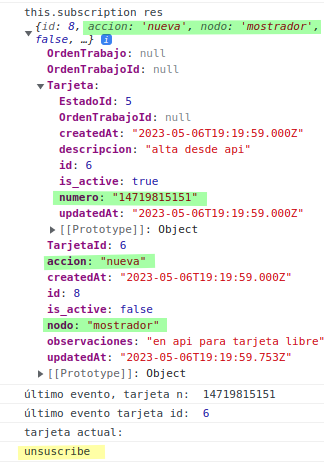
\includegraphics[scale=.60]{./Figures/ensayo-1/5.nueva-2.png}
	\caption{Sección \textit{debub} del navegador.}
	\label{fig:ensayonueva1-2}
\end{figure}

Resaltado en amarillo podemos observar que la suscripción del observador se realizó correctamente cuando hicimos clic en ``LEER TARJETA``. Después pasamos la tarjeta RFID por el lector. 

En verde observamos los datos de la tarjeta leída. Como datos importantes podemos resaltar:

\begin{enumerate}
\item acción = \textit{nueva}.
\item nodo = \textit{mostrador}.
\item número = 14719815151.
\end{enumerate}

Por último podemos leer \textit{unsuscribe} resaltado en color amarillo lo cual indica que la desuscripción del observador se realizó con éxito una vez concluida la lectura de la tarjeta. 

A continuación, en la figura \ref{fig:ensayo-nueva-logs} observamos el log de la API \textit{backend}. 

\begin{figure}[H]
	\centering
	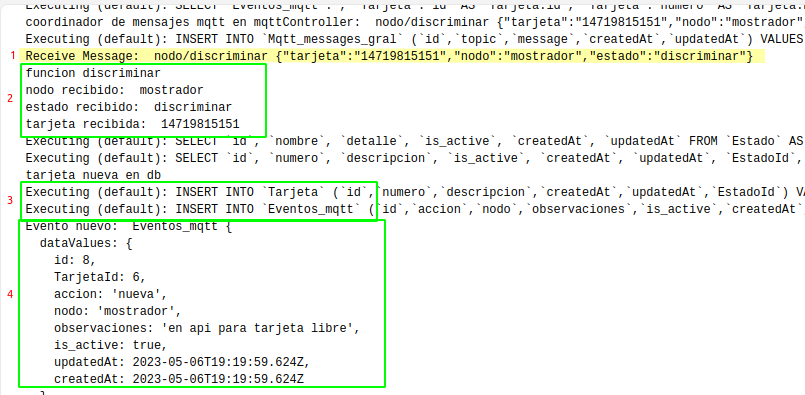
\includegraphics[scale=.60]{./Figures/ensayo-1/6.nueva-logs-1.png}
	\caption{Log API \textit{backend}.}
	\label{fig:ensayo-nueva-logs}
\end{figure}

A fines de poder explicar mejor el registro se enumeraron los puntos importantes y se detallan a continuación:

\begin{enumerate}
\item \textit{Receive Message} se refiere a la recepción del mensaje por MQTT en la API. Se detalla el tópico \textit{nodo/discriminar} que indíca que el mensaje proviene de un nodo y que la acción a ejecutar es discriminar, la cual se verifica en el código fuente por medio de funciones condicionales. El cuerpo del mensaje en formato JSON indíca  el número de la tarjeta, el nombre del nodo, en este caso \textit{mostrador} y el \textit{estado} que indíca que acción se debe tomar.

\item Dentro del recuadro resaltado en verde tenemos los datos anteriormente detallados, los cuales se imprimen en el \textit{log} para una mejor lectura.

\item En este punto tenemos las funciones de insertar en la base de datos dentro de las tablas \textit{Tarjeta} y \textit{Eventos mqtt} los respectivos campos. En la tabla \textit{Tarjeta} se registran los datos de la misma ya que es una tarjeta que no existe previamente en la base de datos, su estado será \textit{libre} hasta que se confirme el ingreso de la órden. En la tabla \textit{Eventos mqtt} se registra que ingresó una tarjeta libre, mediante este registro el observador de Ionic tomará los datos de la tarjeta para insertarlos en el formulario para nueva órden de trabajo.

\item En este recuadro vemos la información detallada que se ingresó en la tabla \textit{Eventos mqtt}, podemos observar que tiene la relación a el ID de la tarjeta, la acción \textit{nueva} y el nodo \textit{mostrador}.
\end{enumerate}

Los próximos pasos que se ejecutan son los de agregar los datos del cliente y la moto para la órden de trabajo, verificando el correcto funcionamiento de los formularios correspondientes. Además completamos el campo \textit{detalle} y \textit{costos}.

Una vez completado el formulario hacemos clic en \textit{Guardar y Limpiar} y confirmamos la operación.

En la figura \ref{fig:ensayonueva10} podemos observar los registros en la consola del navegador web.

\begin{figure}[H]
	\centering
	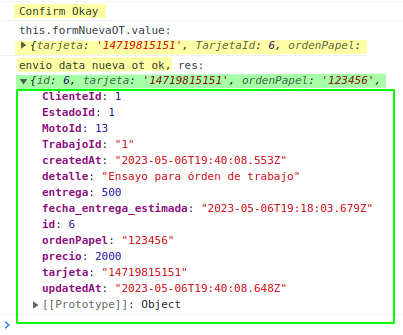
\includegraphics[width=\textwidth]{./Figures/ensayo-1/10.nueva-res.png}
	\caption{Consola del navegador web.}
	\label{fig:ensayonueva10}
\end{figure}

Resaltado en amarillo podemos ver que luego de la confirmación se enviaron correctamente los datos en formato JSON. Luego, en verde, vemos los datos recibidos desde la API, lo cual indica que se procesó la petición correctamente. En la respuesta vemos los datos que fueron cargados en la base de datos, los datos del módelo órden de trabajo y los ID de los modelos que tienen relacion con este registro.

En la figura \ref{fig:ensayonueva10-2} podemos ver el \textit{log} de la API.

\begin{figure}[H]
	\centering
	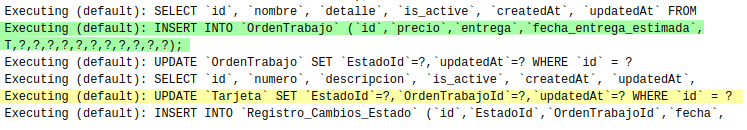
\includegraphics[width=\textwidth]{./Figures/ensayo-1/10.nueva-api-log.png}
	\caption{\textit{Logs} de la API.}
	\label{fig:ensayonueva10-2}
\end{figure}

Resaltamos en verde el proceso que inserta los registros en la base de datos en el modelo \textit{OrdenTrabajo}. En amarillo vemos el proceso que actualiza los datos de la tarjeta, principalmente se actualiza su estado a \textit{en uso} y se la relaciona a la órden de trabajo creada.

Finalmente navegamos en la aplicación web hacia la pestaña \textit{Listado} donde podemos verificar la órden creada. En la figura \ref{fig:ensayolistado} podemos ver, resaltado en amarillo, el nuevo registro y a la derecha, resaltado en verde, podemos verificar en la consola del navegador web que el observador de Ionic se inició correctamente. Este observador se encarga de las actualizaciones de estado de las órdenes que vemos en pantalla.

\begin{figure}[H]
	\centering
	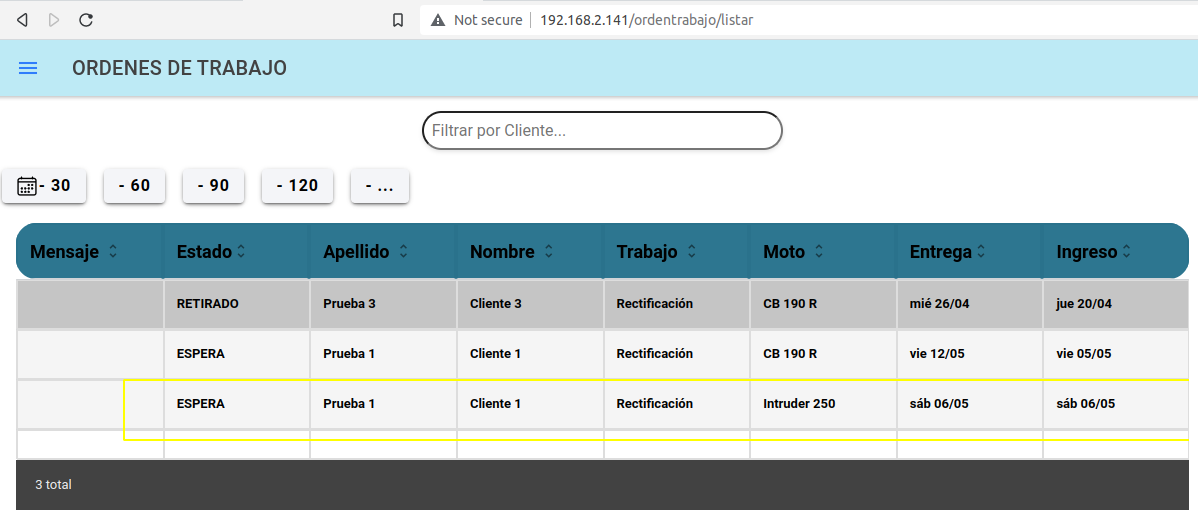
\includegraphics[width=\textwidth]{./Figures/ensayo-1/11.listado.png}
	\caption{Listado de órdenes de trabajo.}
	\label{fig:ensayolistado}
\end{figure}

\subsection{Cambio a estado proceso}
\label{subsec:ensayoaproceso}

En esta sección verificamos el cambio de estado de la órden de trabajo creada previamente. Asignaremos el estado \textit{en proceso}.

Pasamos la tarjeta RFID correspondiente a la órden de trabajo creada en la sección previa por el nodo \textit{proceso} y verificamos los resultados en el log de la API \textit{backend}.

En la figura \ref{fig:ensayolistado} podemos observar los resultados del \textit{log}.

\begin{figure}[H]
	\centering
	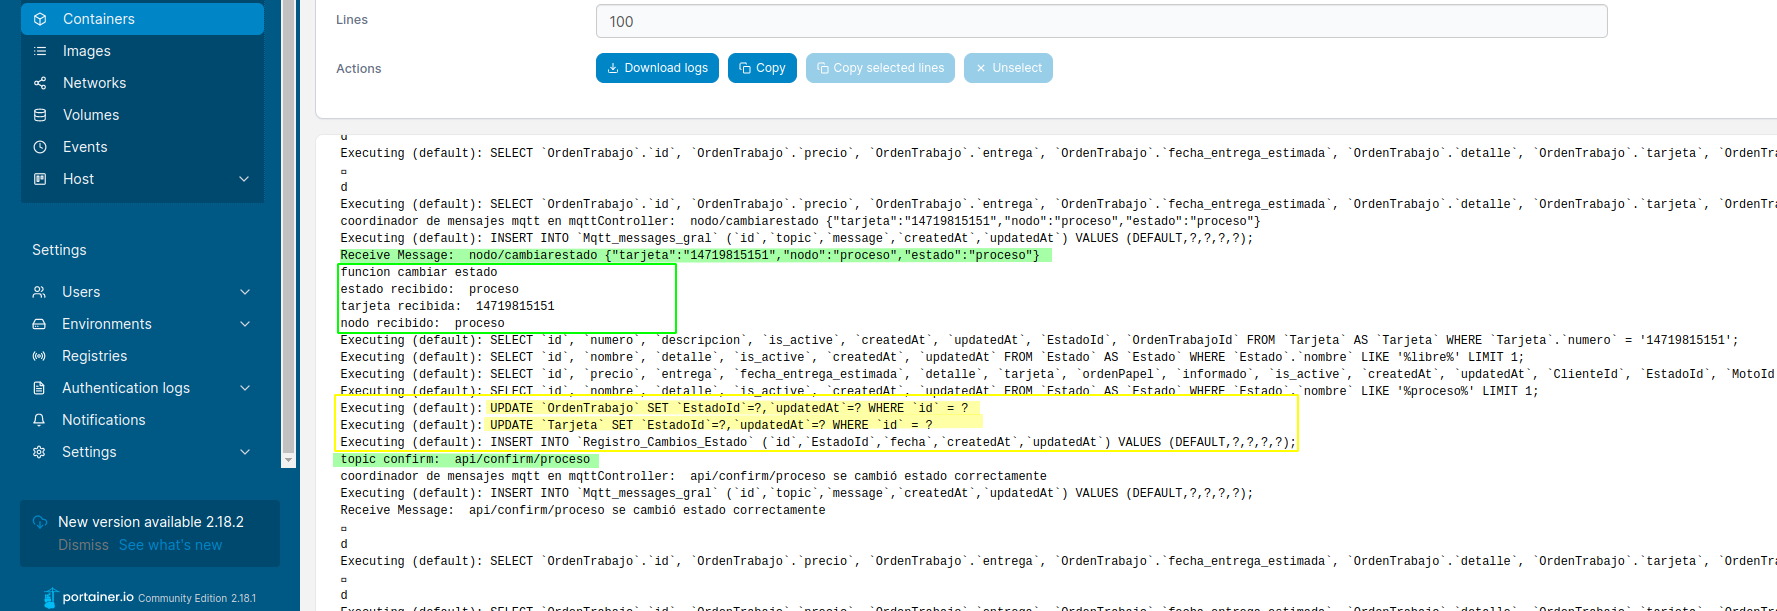
\includegraphics[width=\textwidth]{./Figures/ensayo-1/12.cambioestado-api-log.png}
	\caption{\textit{Logs} de API en cambio de estado.}
	\label{fig:ensayolistado}
\end{figure}

En color verde vemos los registros referentes a la comunicación MQTT, en la primer línea resaltada vemos la recepción del mensaje indicada con el mensaje \textit{Receive Message} y los detalles del mismo donde indica el número de tajeta, el nodo emisor y el estado o acción a ejecutar.

Luego tenemos resaltado en amarillo las líneas que indícan los procesos sobre la base de datos, en este caso son dos actualizaciones o \textit{UPDATES}, una sobre la tabla \textit{OrdenTrabajo} y la otra sobre la tabla \textit{Tarjeta}, en ambas se actualiza el estado utilizando al relación con la tabla \textit{Estado}.

Por último vemos la línea resaltada en verde que indíca el envío de un mensaje de confirmación MQTT al nodo emisor para que se realice el alerta sonoro correspondiente.

Navegamos a la pantalla \textit{Listado} de la aplicación \textit{web} y verificamos el cambio de estado. En la figura \ref{fig:ensayolistado} podemos observar el resultado. La órden a sido actualizada a estado \textit{PROCESO} y cambió el color de la fila correspondiente.

\begin{figure}[H]
	\centering
	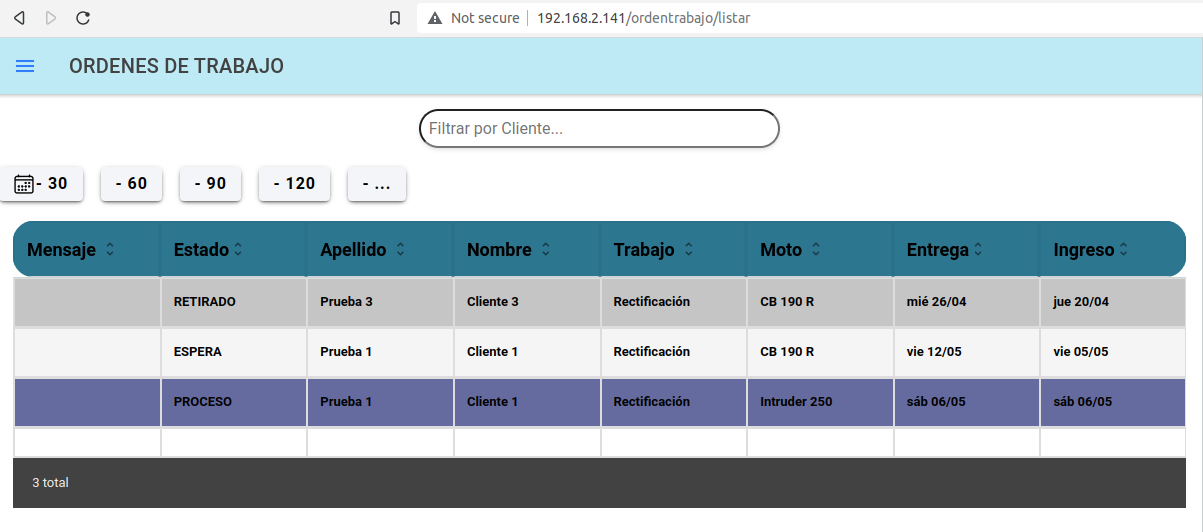
\includegraphics[width=\textwidth]{./Figures/ensayo-1/12.cambioestado-listado.png}
	\caption{Listado de órdenes de trabajo}
	\label{fig:ensayolistadoweb}
\end{figure}

\subsection{Cambio a estado finalizado}
\label{subsec:ensayoafinalizado}

En esta sección verificamos el cambio de estado de la órden de trabajo al estado \textit{finalizado}.

Siguiendo el procedimiento pasamos la tarjeta RFID correspondiente por el nodo \textit{finalizado} y verificamos los resultados en el log de la API \textit{backend}.

En la figura \ref{fig:ensayofinalizadoapi} vemos el l\textit{log}.

\begin{figure}[H]
	\centering
	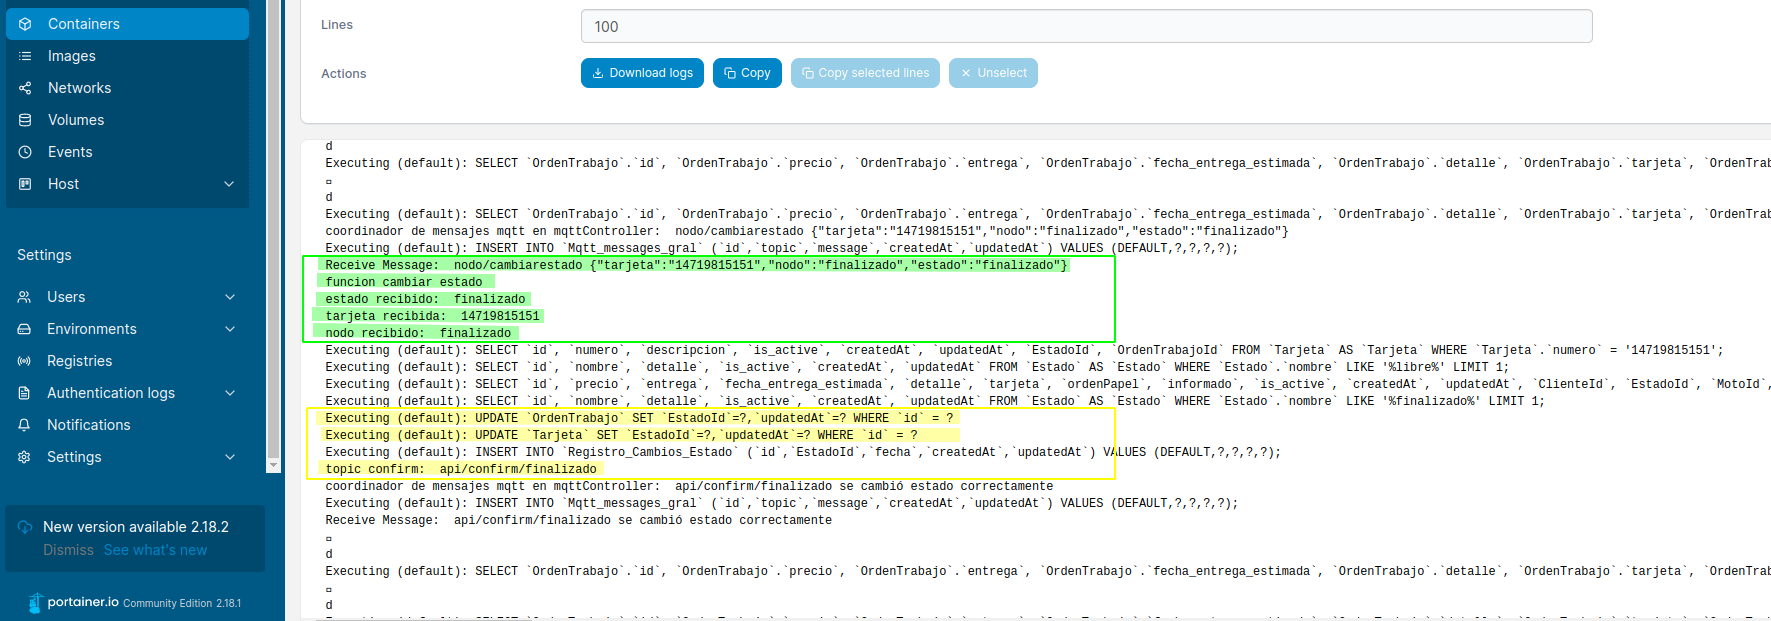
\includegraphics[width=\textwidth]{./Figures/ensayo-1/13.finalizado-api-logs.png}
	\caption{\textit{Logs} de Api en finalizado.}
	\label{fig:ensayofinalizadoapi}
\end{figure}

Vemos resaltado en verde la confirmación de la recepción del mensaje MQTT en el tópico nodo/cambiarestado, con el cuerpo del mensaje en formato JSON. En este caso el estado es finalizado, lo que indica a que estado debe cambiar la órden de trabajo.

En amarillo resaltamos los procesos sobre la base de datos, nuevamente se realiza \textit{UPDATE} en las tablas \textit{OrdenTrabajo} y \textit{Tarjeta} en el campo \textit{EstadoId} que es la clave foranea de la tabla \textit{Estado}.

Por último se envía la confirmación por MQTT al nodo receptor, en este caso el nodo \textit{finalizado}.

En la figura \ref{fig:ensayofinalizadolistado} vemos la aplicación \textit{web} en la sección \textit{Listado}, podemos confirmar el cambio de estado correspondiente en la tabla, el cambio de color de la fila y la correcta visualización del botón con el logo de la aplicación de mensajería.

\begin{figure}[H]
	\centering
	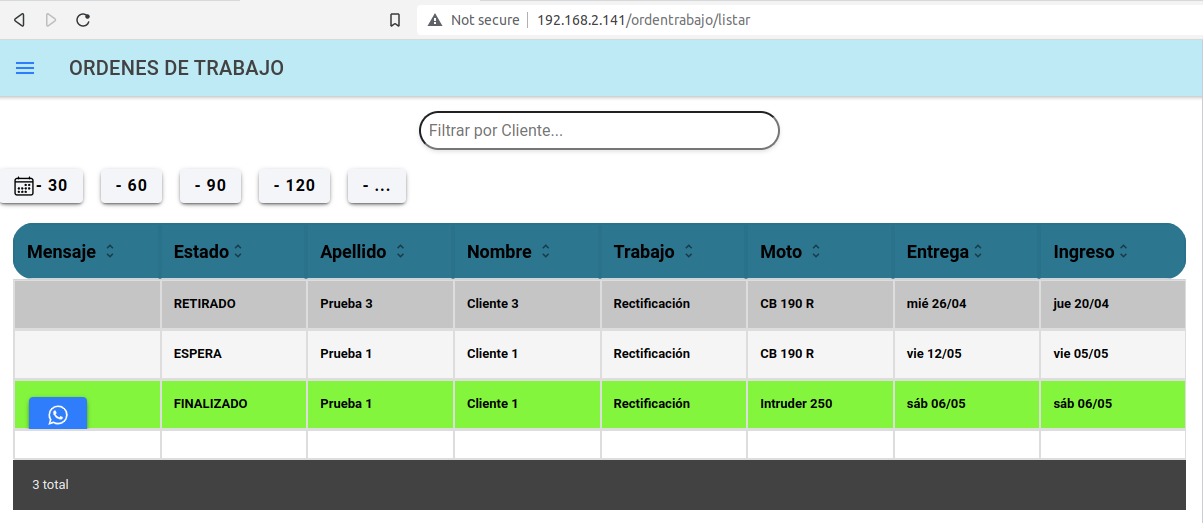
\includegraphics[width=\textwidth]{./Figures/ensayo-1/14.finalizado-listado.png}
	\caption{Listado de órdenes de trabajo.}
	\label{fig:ensayofinalizadolistado}
\end{figure}


\subsection{Envío de mensaje de texto}
\label{subsec:ensayomensaje}

Verificamos la autenticación al servicio de mensajería a través del código QR. 

En la aplicación \textit{web} ingresamos a la sección QR, primero hacemos clic en \textit{Actualizar} para verificar la funcion para renovar el código QR y luego escaneamos el código con un \textit{smartphone}.

En la figura \ref{fig:ensayoqr} vemos la interfaz que muestra el botón para actualizar el código QR y el código correspondiente. 

\begin{figure}[H]
	\centering
	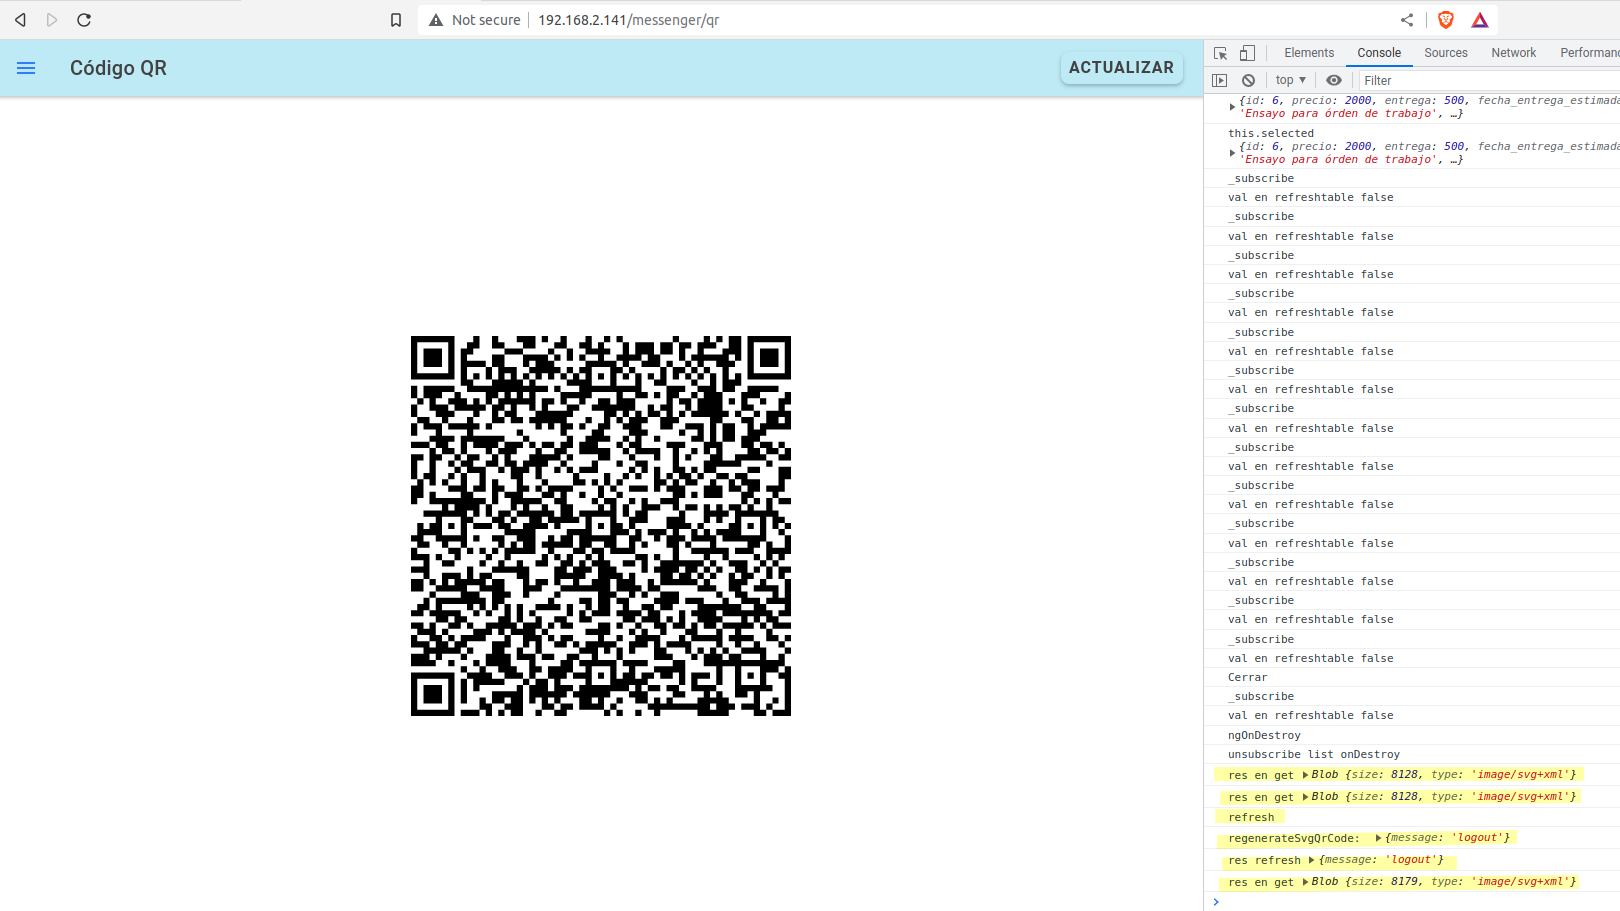
\includegraphics[width=\textwidth]{./Figures/ensayo-1/15.qr.png}
	\caption{Interfaz de código QR.}
	\label{fig:ensayoqr}
\end{figure}

En la figura \ref{fig:ensayomensaje1} observamos el resultado de una correcta autenticación. Debido a que la API de mensajería utiliza una biblioteca del navegador \textit{Google Chrome}, en el listado aparece este navegador como dispositivo vinculado.

\begin{figure}[H]
	\centering
	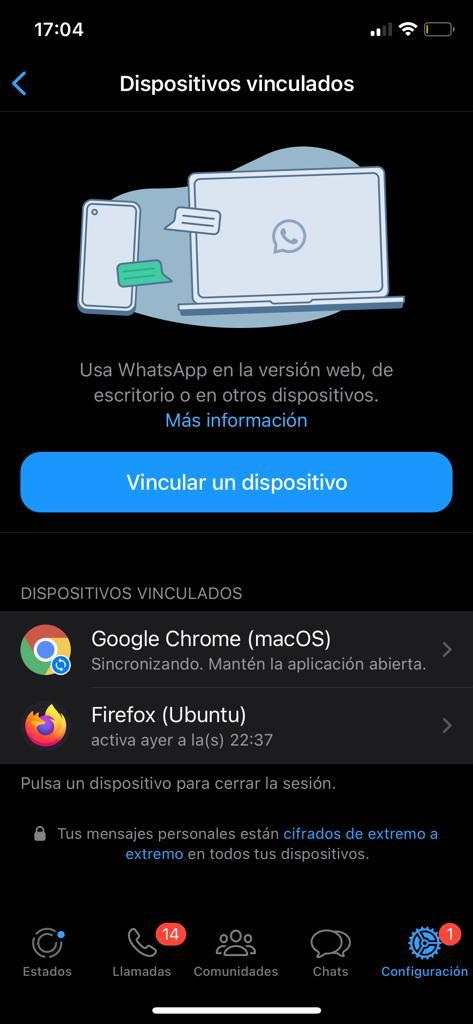
\includegraphics[scale=.20]{./Figures/ensayo-1/15.qr-api.jpeg}
	\caption{Vinculación a \textit{Whatsapp} desde un \textit{Smartphone}}
	\label{fig:ensayomensaje1}
\end{figure}

En la figura \ref{fig:ensayomensajeapi} podemos observar el \textit{log} de la API \textit{Messenger} donde indica, resaltado en amarillo, un primer logout referente a la actualización del código QR realizada, luego vemos el mensaje \textit{LOGIN SUCCESS} que indica que la autenticación se realizó con éxito.

\begin{figure}[H]
	\centering
	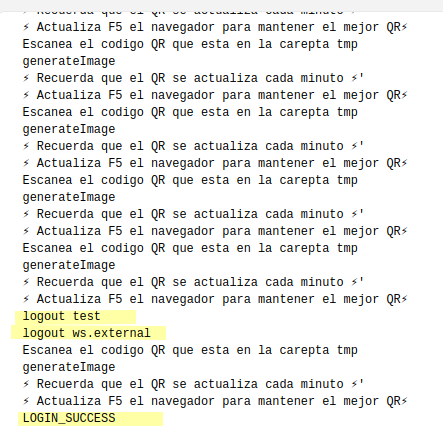
\includegraphics[scale=.70]{./Figures/ensayo-1/15-qr-api.png}
	\caption{\textit{Logs} de API \textit{Messenger}.}
	\label{fig:ensayomensajeapi}
\end{figure}	

En la figura \ref{fig:ensayoconfirmacionmensaje} vemos el modal para confirmación de envío de mensaje.

\begin{figure}[H]
	\centering
	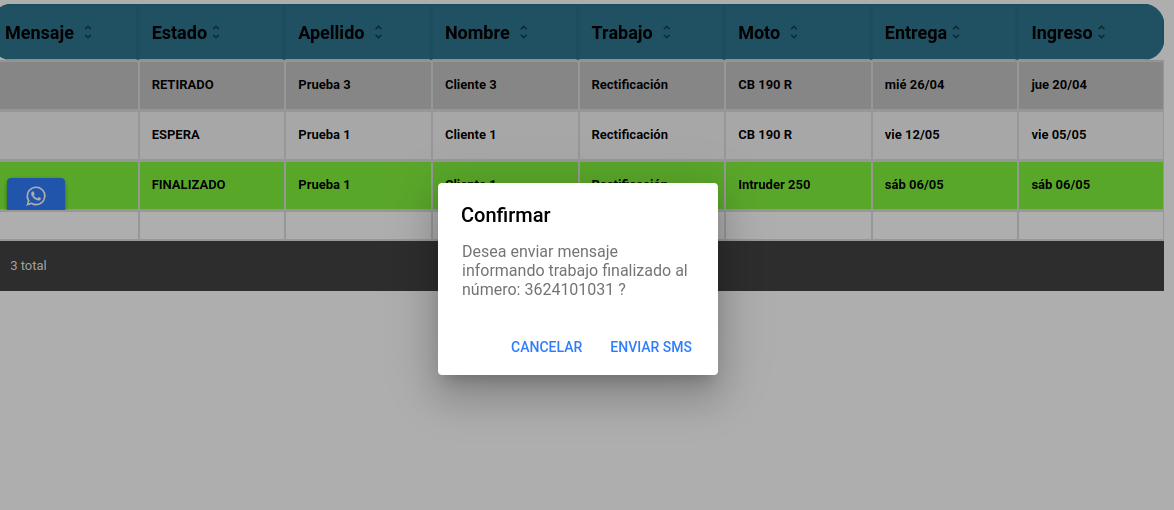
\includegraphics[width=\textwidth]{./Figures/ensayo-1/14.mensaje-confirmacion.png}
	\caption{Confirmación de envío de mensaje.}
	\label{fig:ensayoconfirmacionmensaje}
\end{figure}

En la figura \ref{fig:ensayomensajecel2} podemos ver el mensaje recibido.

\begin{figure}[H]
	\centering
	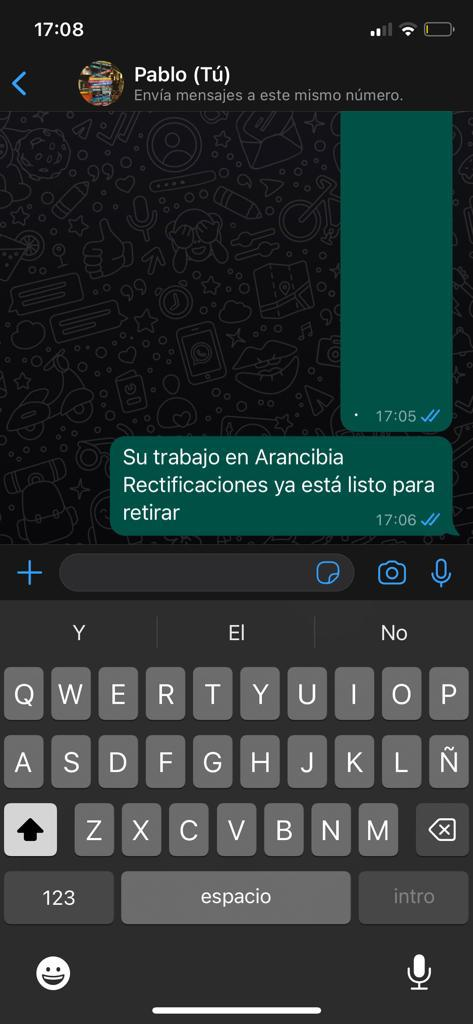
\includegraphics[scale=.20]{./Figures/ensayo-1/15.qr-api-1.jpeg}
	\caption{Mensaje de \textit{Whatsapp} recibido}
	\label{fig:ensayomensajecel2}
\end{figure}

En la figura \ref{fig:ensayomensajefinalizado} observamos el cambio de color a verde opaco de la fila correspondiente. Esto indica que el cliente ya fue informado respecto a su órden de trabajo.

\begin{figure}[H]
	\centering
	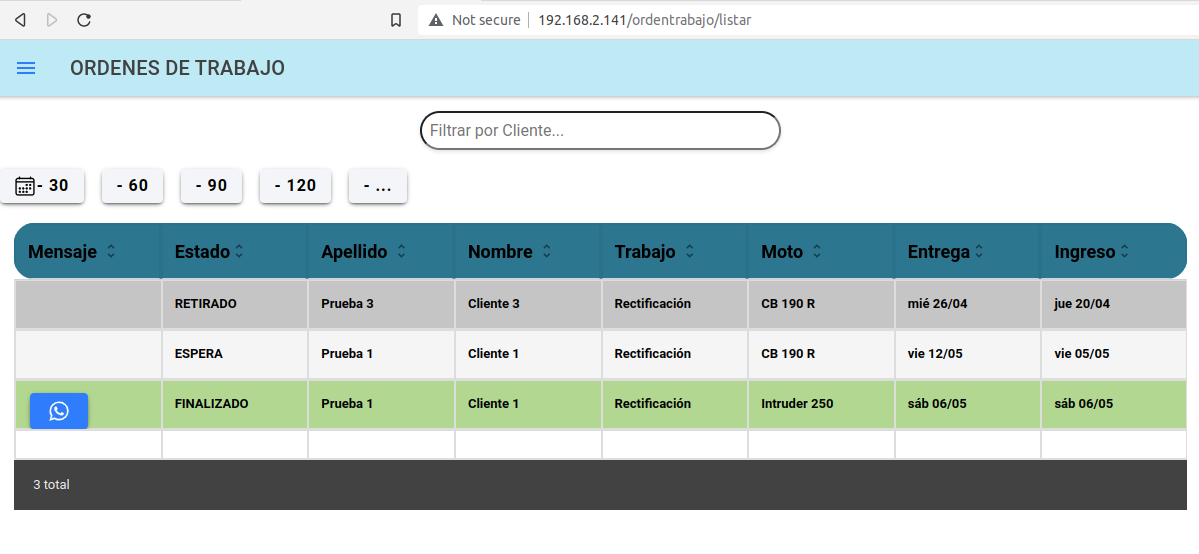
\includegraphics[width=\textwidth]{./Figures/ensayo-1/17.finalizado.png}
	\caption{Listado de órdenes de trabajo.}
	\label{fig:ensayomensajefinalizado}
\end{figure}

Probamos la funcionalidad de reenvio de mensaje. En este caso nos vuelve a mostrar un modal de confirmación de envío pero con el texto \textit{Reenviar Mensaje}. Confirmamos el mensaje y verificamos en el \textit{smartphone} la recepción. En la figura \ref{fig:ensayomensajecel2} vemos el resultado.

\begin{figure}[H]
	\centering
	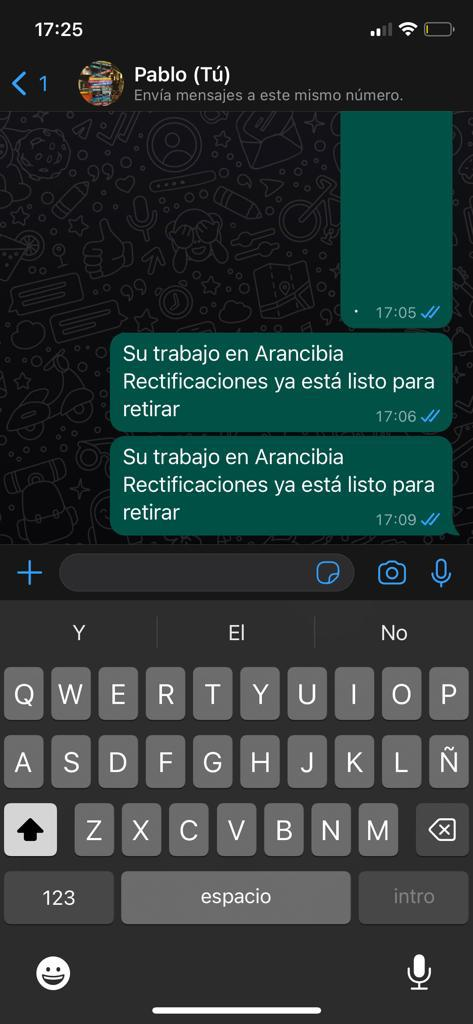
\includegraphics[scale=.20]{./Figures/ensayo-1/15.qr-api-2.jpeg}
	\caption{Mensaje de \textit{Whatsapp} recibido}
	\label{fig:ensayomensajecel2}
\end{figure}

Por último verificamos en la API \textit{backend} el \textit{log} que indica si el cliente fue informado de la finalización de su órden de trabajo.

En la figura \ref{fig:ensayomensajeapilog} vemos resaltada en amarillo la línea que confirma la actualización del campo \textit{informado} en la tabla \textit{OrdenTrabajo}.

\begin{figure}[H]
	\centering
	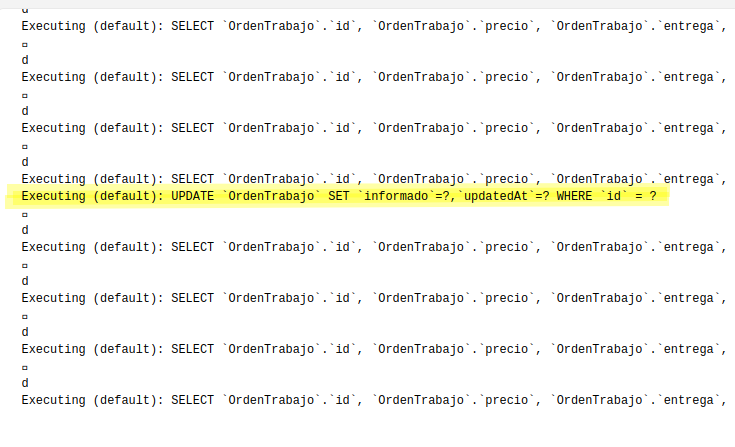
\includegraphics[scale=.50]{./Figures/ensayo-1/20.mensaje-api-log.png}
	\caption{Mensaje de \textit{Whatsapp} recibido}
	\label{fig:ensayomensajeapilog}
\end{figure}


\subsection{Cambio a estado retirado}
\label{subsec:ensayoretiro}

La finalización del ciclo de estados de órdenes de trabajo se da cuando el cliente pasa a retirar su repuesto. En este caso el usuario del sistema debe ingresar a la sección \textit{Retirar} en la aplicación \textit{web}, activar el modo escucha con el botón \textit{Leer Tarjeta} y pasar la tarjeta RFID correspondiente por el nodo mostrador.

En la figura \ref{fig:ensayoretirar-web-1} mostramos la interfaz para retirar una órden de trabajo.

\begin{figure}[H]
	\centering
	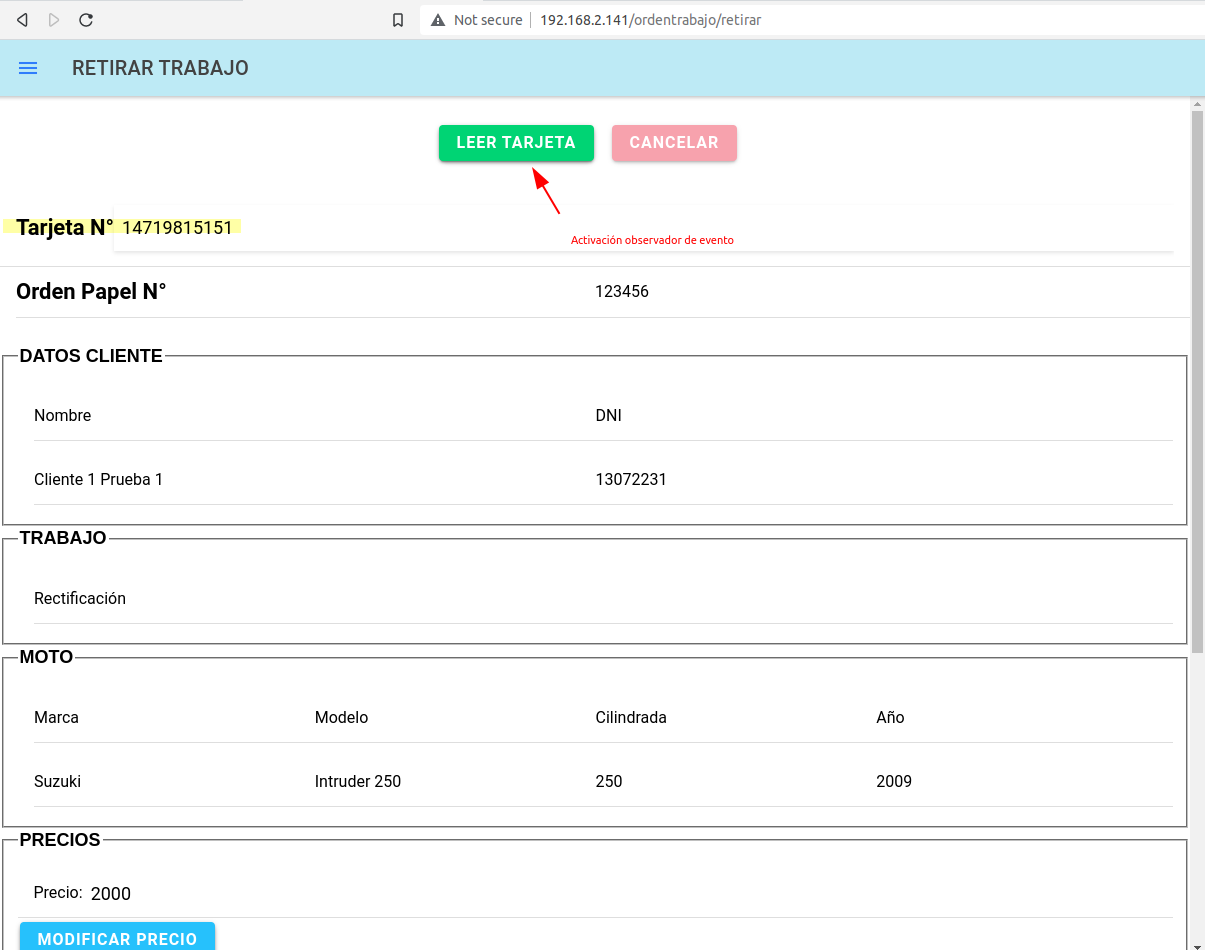
\includegraphics[width=\textwidth]{./Figures/ensayo-1/21.retirar-web-1.png}
	\caption{Interfaz para retirar órden de trabajo.}
	\label{fig:ensayoretirar-web-1}
\end{figure}

En la figura \ref{fig:ensayoretirar-web-2} mostramos la consola del navegador donde podemos observar los datos de la órden de trabajo recibidos desde la API, ya que cuando pasamos la tarjeta por el mostrador la API \textit{backend} recibe y procesa la información y luego esta es leída por la aplicación \textit{web}. Resaltado en verde podemos observar todos los datos de la órden de trabajo y resaltado en celeste podemos ver los datos de la tarjeta. estos datos son insertados en el formulario de retiro.

\begin{figure}[H]
	\centering
	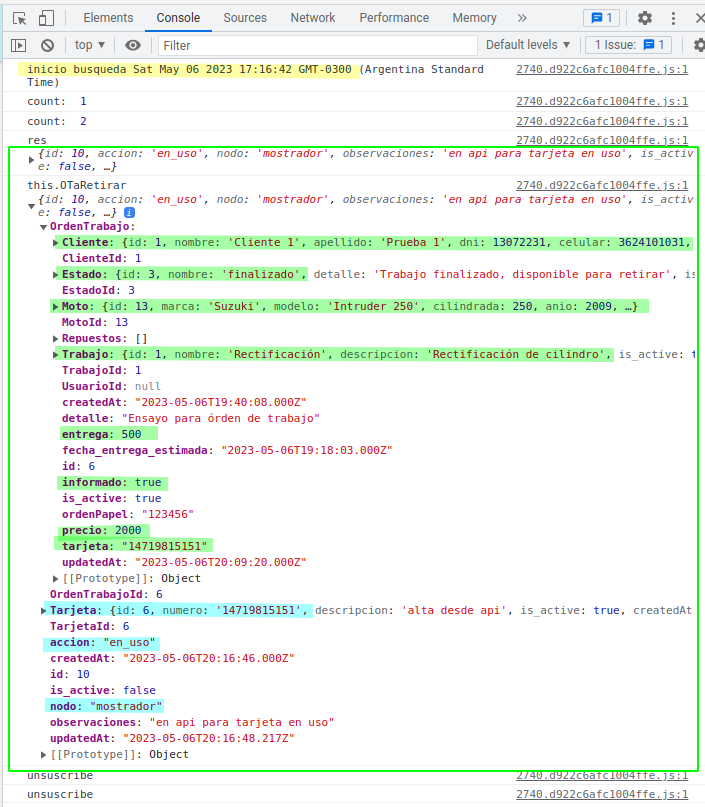
\includegraphics[scale=.50]{./Figures/ensayo-1/21.retirar-web-2.png}
	\caption{Consola de \textit{debug} del navegador.}
	\label{fig:ensayoretirar-web-2}
\end{figure}

En la figura \ref{fig:ensayoretirarapievento} podemos observar los registros en el \textit{log} de la API \textit{backend}. En verde vemos los datos correspondientes a la recepción del mensaje MQTT desde el nodo \textit{mostrador}. Recibimos el número de tajeta y la acción \textit{discriminar}. Luego de procesar la información , resaltamos en amarillo las líneas donde se confirma que se inserta en la base de datos el evento para que luego sea leído por la aplicación \textit{web} y se envía la respuesta por MQTT al nodo emisor, en este caso el nodo \textit{mostrador}.  

\begin{figure}[H]
	\centering
	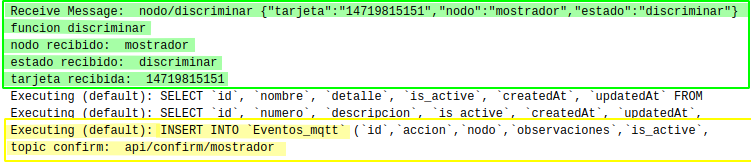
\includegraphics[width=\textwidth]{./Figures/ensayo-1/22.retirar-api-evento.png}
	\caption{\textit{Logs} de recepción MQTT en API \textit{backend}.}
	\label{fig:ensayoretirarapievento}
\end{figure}

Luego que en la aplicación \textit{web} se insertaron los datos de la órden de trabajo, se confirma finalmente el retiro. En la figura \ref{fig:ensayoretirarconfirmacionapi} podemos ver, resaltado en amarillo, los registros en el \textit{log} de la API \textit{backend} pertenecientes a la actualización de la tabla \textit{OrdenTrabajo} y \textit{Tarjeta}. 
 
\begin{figure}[H]
	\centering
	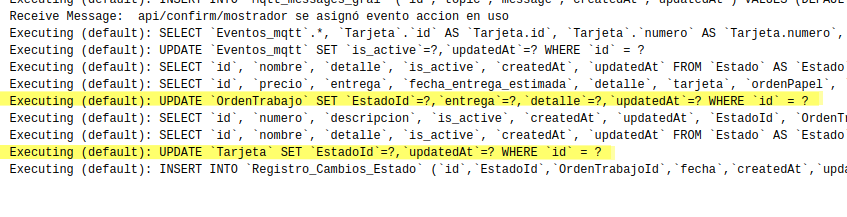
\includegraphics[width=\textwidth]{./Figures/ensayo-1/24.retirar-confirmacion-api.png}
	\caption{\textit{Logs} de confirmación de retiro en API \textit{backend}.}
	\label{fig:ensayoretirarconfirmacionapi}
\end{figure}

De esta manera finaliza el ciclo de una órden de trabajo en el sistema. Pudimos observar en cada paso los resultados y \textit{logs} obtenidos y así asegurar el buen funcionamiento de los diferentes servicios desarrollados e implementados.




